\documentclass[pwidth=11.0in,pheight=8.5in,pcols=4]{posterzine}
% To switch from poster to zine, add 'zine' to the documentclass options


% These are from the article class, but they work here fine when added to a text box
\title{PosterZine}
\author{John T. Murphy}

% This is the only necessary preamble.
\BeginPosterZine

     % You can set options here for the border of each poster/zine panel
     % Options include the border color, whether the border is drawn at all
     % whether graphics inside the border are 'clipped' by it, and whether
     % the border has rounded or straight corners
     \setboxcolor{black}
     \setboxstyle{drawclipstraight}

     % Here are the basic commands to load in text
     % Note that 'AndAdvance' versions finalize the current
     % panel and move to the next one; versions without
     % this can be followed by more commands that add
     % elements to the same panel
     
     % This creates a text box and adds normal LaTeX text to it
     \AddTextElementAndAdvance{
       \maketitle
       
       A {\LaTeX} class that allows you to create posters that are also zines!
     }
     
     % Here is how you can position a graphic
     % Notice that the x and y shifts are in fractions of the panel width
     % (which may be multiple columns), and that the starting point is
     % at the top, so y shifts are negative.
     % The options are derived from includegraphics in the graphicsx
     % package (esp 'set origin', which sets the rotation point to be
     % the center of the image). See notes in the cls file itself

     \setgxshiftfrac{.3}    % fraction across the panel from the left
     \setgyshiftfrac{-.5}   % fraction down from the _top_ of the panel
     \setgpage{1}           % when importing a pdf, can specify the page
     \setgheightfrac{0.6}   % this will re-scale the image to a fraction of the height of the panel
%    \setgwidthfrac{NO!}    % This will not do anything! Graphics are sized relative to the height of the panel; aspect ratio is maintained.
     \setgrotation{0}       % rotate the image about the origin
     
     \AddGraphicElement[2]{Demo1_Poster.pdf}     

     % Modify some of the parameters and add another image
     \setgrotation{-15}
     \setgxshiftfrac{.85}
     \setgyshiftfrac{-.4}
     \AddGraphicElement[2]{Demo1_Zine.pdf}     

     % Positioning text boxes is similar to positioning graphics, except
     % y values are positive here.
     \settextboxfont{\small}
     \settextboxwidthfrac{0.5}
     \settyshiftfrac{.2}          % Note that this is upward from the bottom
     \settxshiftfrac{.3}
     \settextboxfill{pink}
     
     % This allows you to create a text box and then use \input{file} to input a file.
     \AddImportedTextElement[2]{Demo2_Panel2_ImportedText.tex}

     % put all the graphics and text options back to their original values
     \resetgraphicsoptions
     \resettextboxoptions     
     
     \NextPanel[2] % Manually advance to the next panel, just to show it's possible.
                   % Note that we advance 2 panels because the 'panel' we were
                   % on is two columns wide. (And, yes, you could advance just one 
                   % and position elements there...)

     % We can position a different tikz picture, imported from a file
     % Note that we will turn off clipping at the panel edge for this
     \setboxstyle{drawstraight}
     \setgscale{1.2}
     \setgrotation{30}
     \AddImportedTikzElementAt{DemoTikzPicture.tex}{.3}{.3}

     % There's a concern if you turn off clipping that the image will extend
     % across the other panels. Panels already drawn would be overwritten,
     % and panels drawn later will draw over these. You might want this, or you might not.
     % Ways to deal with it include manually clipping it, or drawing the
     % panels in a different order. You can skip to any specific panel
     % by setting the \currentpanelrow and \currentpanelcol counters
     % directly, but be aware that row/column are considered to be the
     % positions in poster mode where (1,1) is at top left and each row
     % goes left to right.

     % Turn clipping back on
     \setboxstyle{drawclipstraight}
     \resetgraphicsoptions     
     
     \settextboxfont{\small}
     \settextboxwidthfrac{0.5}
     \settyshiftfrac{.7}    
     \settextboxfill{red}
     \settrotate{90}

     \AddTextElement{Silly text here!}
     \resettextboxoptions
     
     % This allows you to create a text box and then use \input{file} to input a file.
     % by specifying the x and y shifts on-the-fly, without resetting the global
     % values    
     \AddImportedTextElementAtAndAdvance{Demo2_Panel4_ImportedText.tex}{.4}{.3}
     
     % You can also just import an element; nothing is specified about the
     % positioning or location, so you have to do that in the content
     \AddImportedElement{Demo2_Panel5_ImportedElement.tex}
     \AddTextElementAt{
         Notice that equation counters work:
         
         \begin{equation} 
           S=N\_{eq}^2
         \end{equation}
     }{.4}{.4}
     \NextPanel
     
     % You can use all of the features of include graphics, but only if you
     % eschew the 'ImportedGraphicElement' function above and do it manually.
     
     % One way to do this is verbatim
     \setgheightfrac{.85}
     \setgxshiftfrac{.18}
     \setgyshiftfrac{-0.4}
     \setgpage{1}
     \AddVerbatimElement[2]{
        \begin{scope}[yshift=\zinepanelheight]
          \newlength{\tmpheight} % Note that the 'node' options can do math, but the 'includegraphics' options can't
          \pgfmathsetlength{\tmpheight}{\zinepanelheight * \gheightfrac}
          \node[transform shape, xshift=\gxshiftfrac * \pzptmpPanelWidth, yshift=\gyshiftfrac * \zinepanelheight]
            {\includegraphics[page=\gpage, height=\tmpheight, keepaspectratio]{CarletonEtAl2026.pdf}};
     
          \let\tmpheight\relax
   
        \end{scope}
      
      }
     
     % But you can also do it via import
     % Notice that an imported file has access to many of the temporary variables
     % in the posterzine command of the cls file, but you may also need
     % to define some additional values. If you re-use the imported file,
     % you must define the registers globally and set them for each call.
     % However, defining them here means you don't have access to the posterzine
     % calculated variables (like pzptmpGraphicHeight), so you have to
     % re-calculate them. (Note: Also, some of the documented includegraphics options
     % don't exactly, um, work...)
     \setgxshiftfrac{.78}
     \setgyshiftfrac{-.7}
     \setgpage{12}

     \newlength{\tmpht} % Note that the 'node' options can do math, but the 'includegraphics' options can't; tmpht is used by the imported file
     \pgfmathsetlength{\tmpht}{\zinepanelheight * \gheightfrac}
     \AddImportedElement[2]{Demo2_Panel6_ImportedGraphic1.tex}
     \resetgraphicsoptions
     
     \settextboxfont{\small}
     \settextboxwidthfrac{0.5}
     \settyshiftfrac{.2}          % Note that this is upward from the bottom
     \settxshiftfrac{.3}
     \settextboxfill{pink}
     
     \AddTextElementAndAdvance[2]{
       Standard reference stuff works, too \cite{Carleton_Comparative_2026}.
     }
     \resettextboxoptions


     \settextboxfont{\small}
     \settextboxwidthfrac{0.5}
     \settyshiftfrac{.9}          % Note that this is upward from the bottom
     \settxshiftfrac{.3}
     \settextboxfill{pink}
     
     \AddTextElement{
       Yes, we can produce a reference list.
     }
     
     \settextboxfont{\tiny}
     \settextboxwidthfrac{0.8}
     \settyshiftfrac{.8}          % Note that this is upward from the bottom
     \settxshiftfrac{.1}
     \settextboxfill{white}

     \AddTextElement{
       \bibliographystyle{plain}
       \bibliography{references}
     }
     
     \AddVerbatimElementAndAdvance{\fill[color=red ] circle (2.0); }

\EndPosterZine
